Scopo dell'algoritmo CUTE è la ricerca di pattern di movimento aventi caratteristiche di rilevanza rispetto al percorso e dimensione del gruppo in movimento.
Essendo CUTE un framework generico, deve essere possibile distinguere le varie tipologie di pattern di movimento (swarm, flock, platoon) e verificare le variazioni nel numero degli itemset.
Intuitivamente, una ricerca di swarm produrrà molti più itemset validi di una di flock, per via dei vincoli più rilassati.
Allo stesso modo i diversi livelli di grana delle celle dovranno produrre risultati diversi a seconda delle soglie di supporto e dimensioni.
Per condurre questi test, il dataset utilizzato è stato Geolife, in quanto compatibile con le scale settimanale e giornaliera.

Primo e fondamentale ambito di testing è stato il sistema di riferimento e di conseguenza la granularità di ogni cella.
Questo parametro risulta particolarmente interessante: in un algoritmo di row enumeration, come CUTE o Carpenter, il numero di transazioni determina la complessità dell'algoritmo.
Come detto nella \cref{sec:cute:cim}, nel primo passo della ricerca dei gruppi, ogni cella corrisponde a una transazione.
A seconda del valore dei parametri \(s\) e \(t\), ovvero l'intervallo spaziale e quello temporale, il volume di ogni cella e il loro numero complessivo cambia.
Le \cref{fig:chap-4:cells} mostra il numero di celle al variare del lato \(s\) tra \(1,5,10\)KM.
All'aumentare del lato spaziale delle celle, la compressione dello spazio di ricerca aumenta, diminuendo quindi il numero di celle.
La \cref{fig:chap-4:cellt} mostra invece il rapporto tra \(t\) che varia su \(24h,7gg\) e in assenza di dimensione temporale e le celle. 
Com'è possibile vedere, il numero delle celle a parità di spazio non cresce esponenzialmente, ma di un fattore moltiplicativo collegato ai possibili valori dell'intervallo temporale.

\begin{figure}
  \centering
  \begin{subfigure}{.5\textwidth}
  \centering
   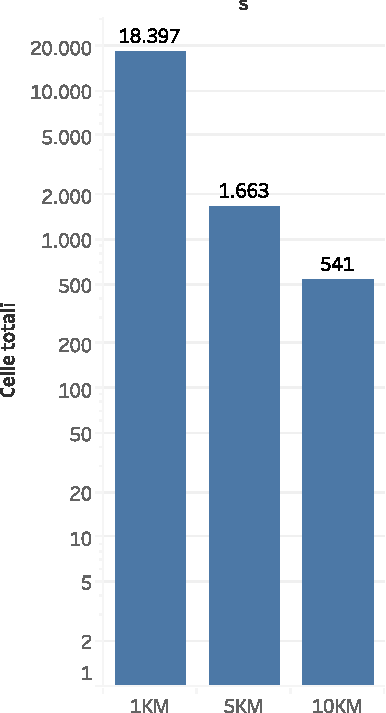
\includegraphics[scale=0.5]{res/fig/sec-4/Cells.pdf}
   \caption{\(s\) tra \(1,5,10\) KM}
  \label{fig:chap-4:cells}
\end{subfigure}%
\begin{subfigure}{.5\textwidth}
  \centering
   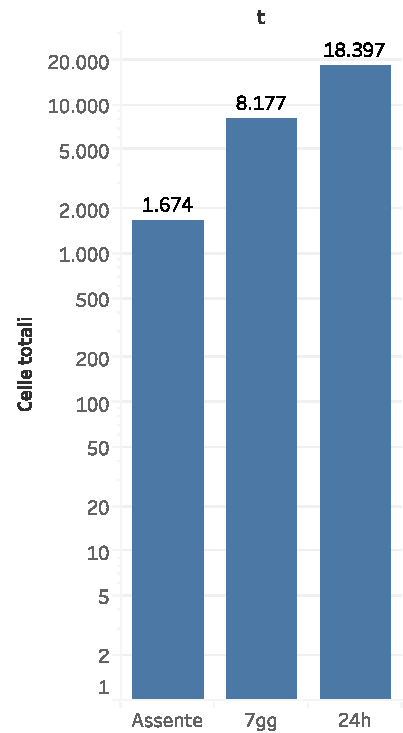
\includegraphics[scale=0.5]{res/fig/sec-4/CellT.pdf}
   \caption{\(t\) tra 24h, 7gg e assenza di tempo}
  \label{fig:chap-4:cellt}
\end{subfigure}%
  \caption{Celle alla variazione di \(s\) a sinistra, \(t\) a destra}%
  \label{fig:chap-4:cellst}
\end{figure}

Su ognuna delle configurazioni sopra espresse è stata eseguita una ricerca di itemset rispetto alle variazioni dei parametri in gioco presentati nella \cref{subsec:cute:params}.
I valori espressi per questi parametri sono riassunti nella \cref{tab:parameters-variation}.
Nei successivi test, dove non specificato, ai parametri è assegnato il valore di default (in grassetto nella \cref{tab:parameters-variation}).

\begin{table}[H]
    \centering
   \begin{tabular}{||c c c||}
 \hline
     Param. & Significato & Valori \\ [0.4ex] 
 \hline\hline
   s & Lato spaziale cella & \textbf{1KM}, 5KM, 10KM \\
   \hline
   t & Lato temporale cella & \textbf{24h}, 7gg, assenza di tempo \\
   \hline
   minsize & dimensione dei gruppi & 5, \textbf{10}, 15 \\
   \hline
   minsup & supporto minimo & 5, \textbf{10}, 15 \\
   \hline
   \(\epsilon\) & soglia spaziale & 2, \textbf{5}, 10, \(\infty\) \\
   \hline
   \(\tau\) & soglia temporale & 1, \textbf{2}, \(\infty\) \\
 \hline
\end{tabular}
    \caption{Parametri e il loro valore di default (in grassetto)}
    \label{tab:parameters-variation}
\end{table}

In particolare il focus di questi test è capire come varia il numero dei cluster individuati all'interno del problema.
I valori di supporto e dimensione minima coincidono e sono stati determinati empiricamente.
Il range di \(\epsilon\) varia tra \((2, 5, 10, \infty)\) mentre quello di \(\tau\) tra \((1, 2, \infty)\).
Mentre i valori di \(\epsilon\) sono stati scelti sperimentalmente, quelli di \(\tau\) sono stati selezionati sulla base del range delle scale temporali utilizzate.
In particolare le scale giornaliere e settimanale presentano una natura ciclica.
Una scala ciclica non ha un valore massimo assoluto e un minimo assoluto, ma prevede che il valore successivo al massimo sia il minimo.
Questa circolarità impatta la misura della distanza tra due punti.
Questa è definita come la dimensione del più piccolo intervallo tra due punti: può essere quindi la minima distanza calcolata dal maggiore al minore o viceversa.
Ciò comporta che all'interno di una scala ciclica, i valori siano molto più vicini rispetto a una monotona.
Quindi è molto facile che considerando valori alti di \(\tau\) il risultato tenda a essere quello di \(\tau = \infty\).
Ciò vale soprattutto per la scala settimanale: essendo solamente \(7\) i giorni della settimana e la scala ciclica per definizione, la distanza massima tra due qualunque elementi è al massimo \(3\).
Questo implica che l'unico valore plausibile per eseguire una ricerca di platoon su questa scala sia \(2\).
\(\tau\) determina inoltre la categoria di co-movement pattern individuato, ad esempio su scala settimanale vale che:
\begin{itemize}
    \item \(\tau = 1\): Flock
    \item \(\tau = 2\): Platoon g-connected
    \item \(\tau = \infty\): Swarm
\end{itemize}

\begin{figure}
  \centering
  \begin{subfigure}{.5\textwidth}
  \centering
   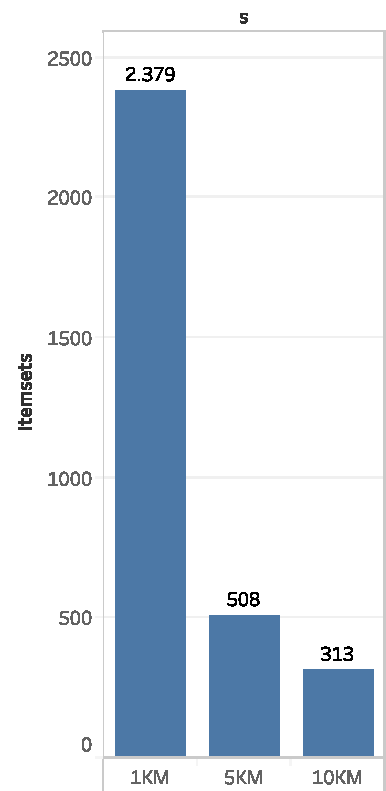
\includegraphics[scale=0.5]{res/fig/sec-4/itemset/ItemsetS.pdf}
   \caption{\(s\) tra \(1,5,10\) KM}
  \label{fig:chap-4:ItemsetS}
\end{subfigure}%
\begin{subfigure}{.5\textwidth}
  \centering
   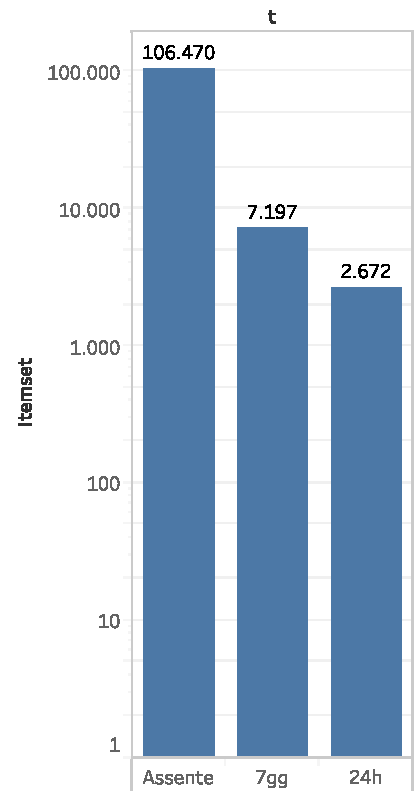
\includegraphics[scale=0.5]{res/fig/sec-4/itemset/ItemsetT.pdf}
   \caption{\(t\) tra 24h, 7gg e assenza di tempo}
  \label{fig:chap-4:ItemsetT}
\end{subfigure}%
  \caption{Numero di itemset alla variazione di \(s\) a sinistra, \(t\) a destra}%
  \label{fig:chap-4:ItemsetSandT}
\end{figure}

Le \cref{fig:chap-4:ItemsetS,fig:chap-4:ItemsetT} mostrano le variazioni del numero di itemset su \(s\) e \(t\).
Per quanto riguarda le variazioni nel lato spaziale delle celle \(s\), i risultati sono coerenti con quanto atteso: all'aumentare dell'area coperta dalle celle, calano il numero di itemset individuati (\cref{fig:chap-4:ItemsetS}).
Ciò è coerente con la natura del problema: se ogni cella corrisponde a una transazione, al calare del numero di transazioni a parità di supporto calano sia il numero di itemset frequenti che il tempo necessario per eseguire la ricerca.
Per \(t\), i risultati presentati sono stati ottenuti ponendo \(\tau = \infty\), questo perché non avrebbe avuto senso considerare la continuità nel tempo considerando una scala come l'assenza di tempo che esclude questa dimensione (\cref{fig:chap-4:ItemsetT}).
Alla luce di ciò, la dimensione temporale \(t\) presenta invece un trend opposto a \(s\) per quanto riguarda gli itemset individuati: l'impiego della scala giornaliera rispetto a quella settimanale individua meno itemset sia in caso di vincoli su \(\tau\) che in sua assenza.
L'assenza di una dimensione temporale invece produce risultati di circa un ordine di grandezza superiori rispetto agli altri due.
Questo fenomeno può essere direttamente collegato all'aumento del numero di celle a seguito dell'adozione di diverse scale temporali.
L'introduzione di una nuova dimensione produce infatti un'ulteriore suddivisione dello spazio di ricerca: un pattern valido in uno spazio \(n\)-dimensionale può non risultarlo più in uno \(n+1\) dimensionale, poiché il gruppo può non risultare vicino nella nuova dimensione.
Questa frammentazione sarà tanto più netta tanti più valori possibili avrà la scala della nuova dimensione.
Applicando quanto detto sopra alle scale temporali, l'assenza di tempo non produce nessuna ulteriore divisione, la scala settimanale e quella temporale aggiungono una cardinalità di rispettivamente \(7\) e \(24\) intervalli.
La frammentazione dello spazio di ricerca causa quindi la differenza nei risultati delle tre scale.


Le \cref{fig:chap-4:ItemsetMinsize,fig:chap-4:ItemsetMinsupp} individuano le variazioni di pattern riconosciuti al variare di supporto e dimensione minima.
Minsup e minsize (\(\alpha, \gamma\)) sono fatti variare tra \(5, 10, 15\).
Entrambi i parametri si comportano come atteso: all'aumentare del valore cala il numero di itemset individuati.
La ricerca di gruppi di dimensioni maggiori o che abbiano un elevato tempo di viaggio riduce il numero di itemset validi.

\begin{figure}
  \centering
   \begin{subfigure}{.5\textwidth}
  \centering
    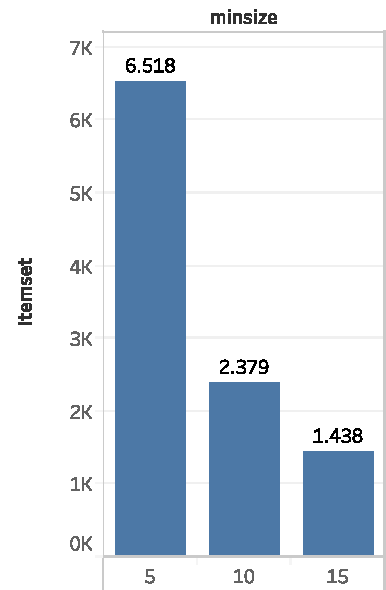
\includegraphics[scale=0.5]{res/fig/sec-4/itemset/ItemsetMinsize.pdf}
   \caption{\(minsize\) tra \(5,10,15\)}
  \label{fig:chap-4:ItemsetMinsize}
\end{subfigure}%
\begin{subfigure}{.5\textwidth}
  \centering
   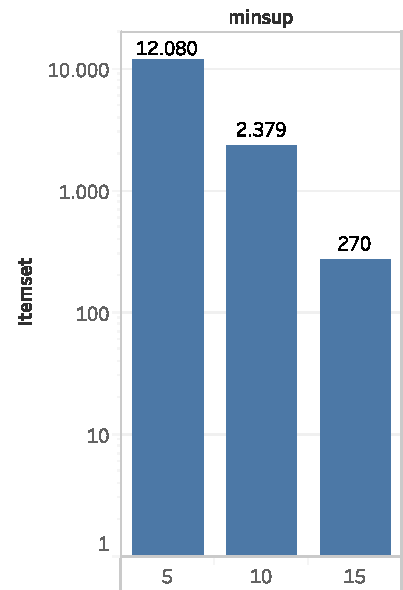
\includegraphics[scale=0.5]{res/fig/sec-4/itemset/ItemsetMinsupp.pdf}
   \caption{\(minsup\)  tra \(5,10,15\)}%
  \label{fig:chap-4:ItemsetMinsupp}
  \end{subfigure}%
  \caption{Numero di itemset alla variazione di \(minsize\) a sinistra e \(minsupp\) a destra}%
  \label{fig:chap-4:ItemsetMinsizeandMinsupp}
\end{figure}

Infine i test condotti su \(\epsilon\) e \(\tau\) mostrano il diverso numero di pattern individuati stringendo o rilassando i vincoli di contiguità.
Per quanto riguarda \(\epsilon\), la \cref{fig:chap-4:ItemsetEpsilon} mostra come il numero di pattern individuati cali al diminuire del valore di soglia.
Questa tendenza rallenta solo nel caso dei valori \(10\) e \(\infty\) dove i risultati quasi coincidono.
I risultati ottenuti su questo parametro sono coerenti con quanto atteso: vincoli più stretti producono meno itemset.
La coincidenza tra il valore \(10\) e \(\infty\) può essere motivata dall'ampiezza del raggio di vicinanza coperto rispetto all'area complessiva del problema.
Un raggio di vicinato pari a \(10\)KM include probabilmente la maggior parte delle celle individuate nello spazio, di conseguenza i suoi risultati tendono a quelli ottenuti rilassando il vincolo.

Per quanto riguarda \(\tau\), è possibile riscontrare come la ricerca di flock, platoon e convoy non produca le differenze attese nei risultati.
Su Geolife le differenze riguardano solo poche tuple tra le tre ricerche.
Questi risultati sono mostrati nella \cref{fig:chap-4:ItemsetTau}.
Questo comportamento è a prima vista inusuale: i vincoli sullo spazio si dimostrano efficaci nella riduzione dello spazio di ricerca mentre quelli sul tempo sono praticamente trascurabili.
Tuttavia occorre considerare la diversità fra la scala spaziale e quella temporale in termini di possibili elementi: quest'ultima infatti ha un range decisamente inferiore rispetto a qualunque scala temporale utilizzata nel corso dei test.
Nel caso di scala giornaliera ad esempio i valori possibili sono \(24\), mentre per quella settimanale sono \(7\).
Come detto nella presentazione di Geolife, i singoli punti hanno frequenze di campionamento molto più elevate della granularità temporale del sistema di riferimento.
Quindi sono poche le traiettorie che hanno una continuità rispetto alle ore del giorno, ancora meno rispetto ai giorni della settimana.

\begin{figure}
  \centering
   \begin{subfigure}{.5\textwidth}
  \centering
    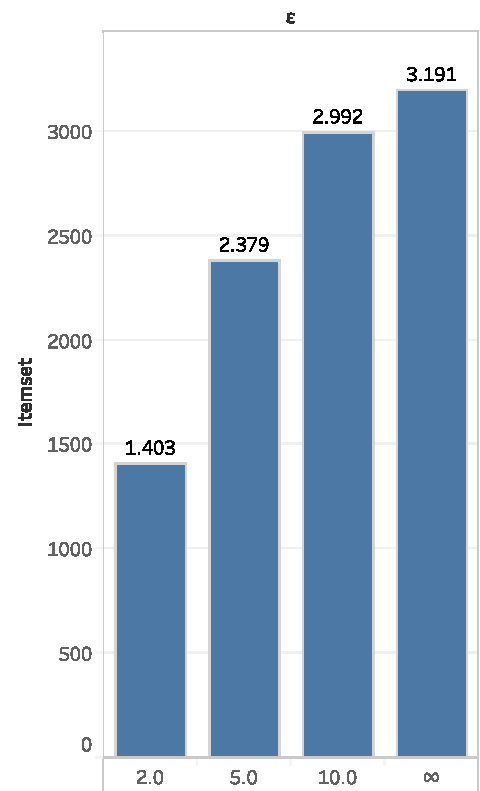
\includegraphics[scale=0.5]{res/fig/sec-4/itemset/ItemsetEpsilon.pdf}
   \caption{\(\epsilon\) tra \(2,5,10,\infty\)}
  \label{fig:chap-4:ItemsetEpsilon}
\end{subfigure}%
\begin{subfigure}{.5\textwidth}
  \centering
   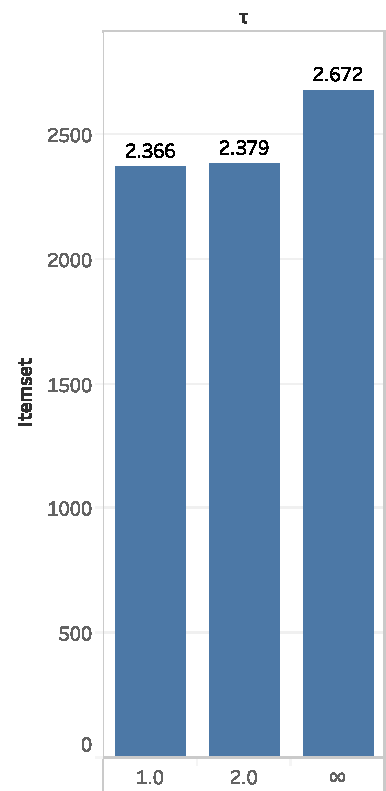
\includegraphics[scale=0.5]{res/fig/sec-4/itemset/ItemesetTau.pdf}
   \caption{\(\tau\) tra \(1,2,\infty\)}%
  \label{fig:chap-4:ItemsetTau}
  \end{subfigure}%
  \caption{Numero di itemset alla variazione di \(\epsilon\) a sinistra e \(\tau\) a destra}%
  \label{fig:chap-4:ItemsetEpsilonAndTau}
\end{figure}


